%\title{LaTeX Portrait Poster Template}
%%%%%%%%%%%%%%%%%%%%%%%%%%%%%%%%%%%%%%%%%
% a0poster Portrait Poster
% LaTeX Template
% Version 1.0 (22/06/13)
%
% The a0poster class was created by:
% Gerlinde Kettl and Matthias Weiser (tex@kettl.de)
% 
% This template has been downloaded from:
% http://www.LaTeXTemplates.com
%
% License:
% CC BY-NC-SA 3.0 (http://creativecommons.org/licenses/by-nc-sa/3.0/)
%
%%%%%%%%%%%%%%%%%%%%%%%%%%%%%%%%%%%%%%%%%

%----------------------------------------------------------------------------------------
%	PACKAGES AND OTHER DOCUMENT CONFIGURATIONS
%----------------------------------------------------------------------------------------

\documentclass[a0,portrait]{a0poster}
\usepackage{fix-cm}
\newcommand\HUGE{\fontsize{80}{100}} 
%\documentclass[]{beamerposter}
%\documentclass[final]{beamer}
%\usepackage[size=custom,width=240,height=120,scale=1.24]{beamerposter} % Use the beamerposter package for laying out the poster
\usepackage{anyfontsize}
\usepackage{multicol} % This is so we can have multiple columns of text side-by-side
\columnsep=100pt % This is the amount of white space between the columns in the poster
\columnseprule=3pt % This is the thickness of the black line between the columns in the poster

\usepackage[svgnames]{xcolor} % Specify colors by their 'svgnames', for a full list of all colors available see here: http://www.latextemplates.com/svgnames-colors

\usepackage{times} % Use the times font
%\usepackage{palatino} % Uncomment to use the Palatino font

\usepackage{graphicx} % Required for including images

\graphicspath{{figures/}} % Location of the graphics files
\usepackage{booktabs} % Top and bottom rules for table
\usepackage[font=large,labelfont=bf]{caption} % Required for specifying captions to tables and figures
\usepackage{amsfonts, amsmath, amsthm, amssymb} % For math fonts, symbols and environments
\usepackage{wrapfig} % Allows wrapping text around tables and figures
\usepackage{helvet}
\renewcommand{\familydefault}{\sfdefault}

%\sectionfont{\fontsize{12}{15}\selectfont}

\begin{document}

%----------------------------------------------------------------------------------------
%	POSTER HEADER 
%----------------------------------------------------------------------------------------

% The header is divided into two boxes:
% The first is 75% wide and houses the title, subtitle, names, university/organization and contact information
% The second is 25% wide and houses a logo for your university/organization or a photo of you
% The widths of these boxes can be easily edited to accommodate your content as you see fit

\definecolor{wpi_red}{RGB}{197, 18, 48}
\vspace*{2cm}
\begin{minipage}[t]{0.7\linewidth}
\veryHuge \color{wpi_red} \textbf{Learning a Protocol for Minimum Probability of Detection Wireless Transmissions: A DQN Experiment}
\color{Black}\\[0.5cm] % Title
%\Huge\textit{Framework For Multi-Core Parallelism}\\[1cm] % Subtitle
\huge \textbf{Mac Carr, Kyle McClintick, Bryan Nguon}\\[0.5cm] % Author(s)
\huge WPI: Wireless Innovation Laboratory\\[0.4cm] % University/organization
\end{minipage}%
\hspace{1cm}
\begin{minipage}[t]{0.3\linewidth}
\strut\vspace*{-\baselineskip}\newline
\includegraphics[width=22cm]{WPI_Inst_Prim_FulClr_cropped.png}\\

\end{minipage}



\begin{multicols}{2} % This is how many columns your poster will be broken into, a portrait poster is generally split into 2 columns

\section{Non-Adversarial Case}
\large

Wireless communications operate under many parameters (PHY) and policies (NET, LINK). Given a few minutes of power, time, and frequnecy data (spectrograms), can an optimal wireless communications policy be learned?


\begin{center}
\center{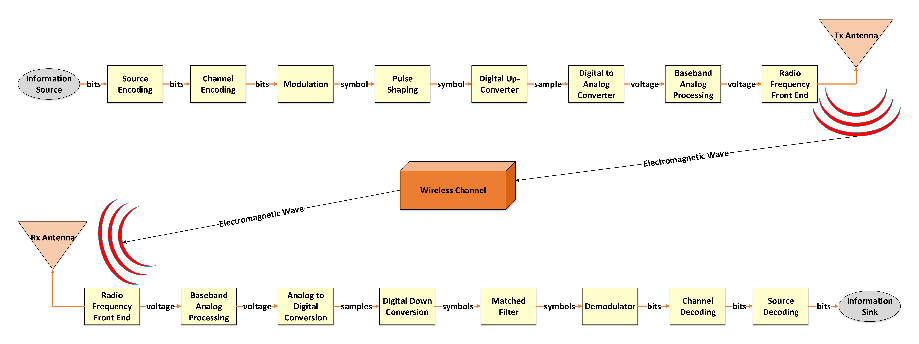
\includegraphics[width=0.48\textwidth]{txrx.eps}}
\captionof{figure}{The sequential model for estimating wirelessly transmitted binary data across a noisy wireless channel}
\end{center}




\begin{align}
BER &= \frac{correct bits}{incorrect bits}
\\
reward &= \log (1 / (BER + \epsilon) )
\\
f_c &\in \{ f_s/10 ,f_s/2  \}
\\
power &\in \{ 0.1, 1.0 \}
\\
action & \in \{ (power, f_c)  \}
\\
state & \in \mathbb{R}^{(BS, 1, 257, 311)}
\end{align}

\vspace{5cm}

\begin{center}
\center{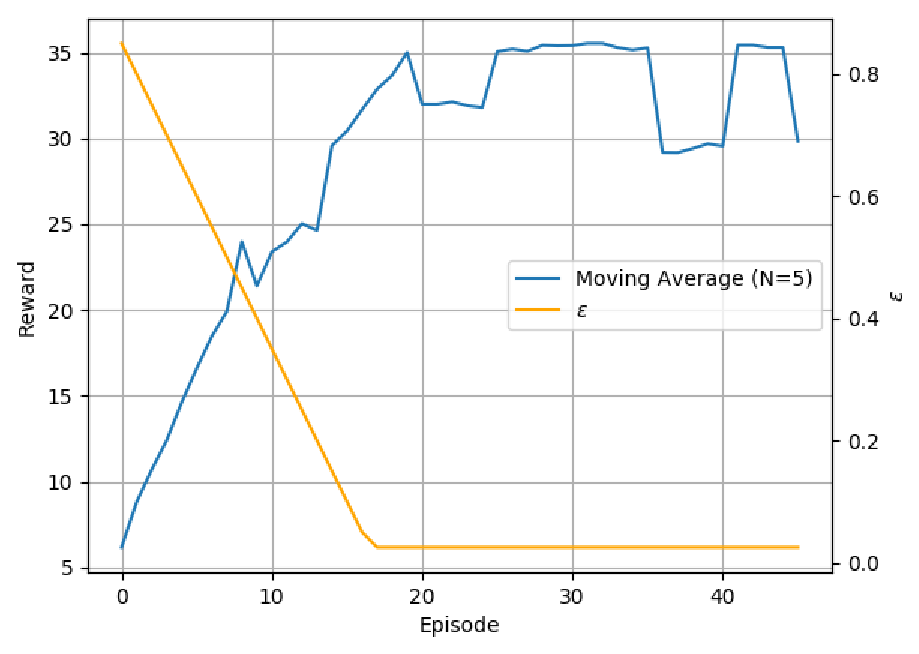
\includegraphics[width=0.45\textwidth]{base_case_rew.eps}}
\captionof{figure}{Training reaches a maximum reward very quickly as exploration ceases in this simple problem. Testing average over 100 episodes gave $31.30$ reward ($\sim 2.5 \times 10^{-14}$ BER)}
\end{center}

\vspace{5cm}

\section{Adversarial Case}

Signal to Interference and Noise Ratio (SINR) is computed as in-band signal power divided by the sum of noise and interference power: $P_s / (P_i + P_n)$. An adversary is assumed to be able to detect our transmission if this ratio exceeds $0 dB$ or a one to one ratio. Can a policy be learned to operate as close to this unknown SINR but not above it?

\vspace{3cm}

\begin{center}
\center{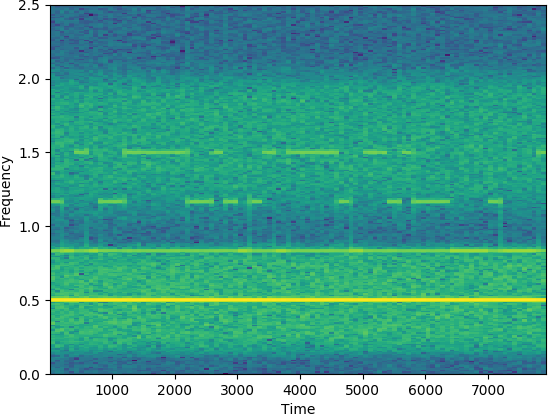
\includegraphics[width=0.45\textwidth]{poster_spec.png}}
\captionof{figure}{An example state with actions chosen $a_t :  \{ (gain=1,f_c=0.5) \}$. Tone exists at $.83 Hz$, hopping tones at $1.16, 1.5 Hz$, and wide band signal from $1.2 Hz$ to $2 Hz$. SINR exceeds $0 dB$, so detection and jamming occurs.}
\end{center}

\vspace{5cm}


\begin{center}
\center{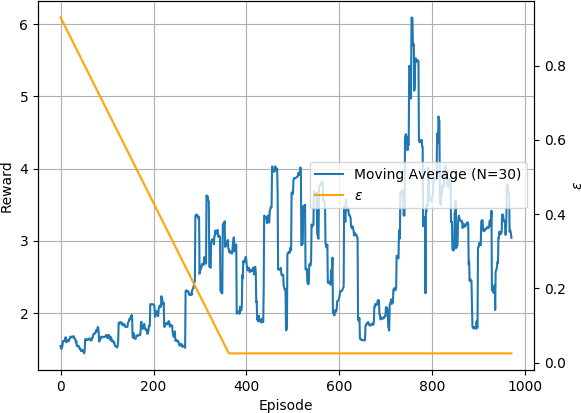
\includegraphics[width=0.45\textwidth]{rew_adversarial.png}}
\captionof{figure}{Training reaches a maximum reward more slowly. Testing average over 100 episodes gave $9$ reward ($\sim 1 \times 10^{-4}$ BER). A larger sliding window for the average is used to capture the smaller margin between good and bad performance ($\sim 1$ and $\sim 5-10$ average reward per time step instead of $\sim 1$ and $\sim 36$ non-adversarial margin). DQN additionally learned to avoid wide band interference, SINR equal.}
\end{center}


\end{multicols}
\vspace{2cm}
\begin{minipage}[b]{0.3\linewidth}
\strut\vspace*{-\baselineskip}\newline
\includegraphics[width=25cm]{wilab_logo.jpg}
\end{minipage}
\hspace{0.01cm}
\begin{minipage}[b]{0.3\linewidth}
\hspace{20mm}
\vspace{10mm}
\color{wpi_red} \textbf{\textsf{\fontsize{138}{60}\selectfont www.Wireless.WPI.edu}}
\end{minipage}
\hspace{16cm}



\end{document}
